\clearpage{\pagestyle{empty}\cleardoublepage}
\chapter{Contesto}
\lhead[\fancyplain{}{\bfseries\thepage}]{\fancyplain{}{\bfseries\rightmark}}
\pagenumbering{arabic}

TODO: descrizione di una pagina sugli argomenti che andremo a trattare in questo capitolo \newpage

\section{Open Data} % : definizione e contesto
Le nuove tecnologie permettono di creare servizi in grado di migliorare la vita dei cittadini e di far funzionare più efficientemente governi e società. Molti dei dati necessari a raggiungere questi obiettivi sono prodotti da organismi pubblici, tuttavia spesso tali dati non sono disponibili in formati che li rendano facili da manipolare. Per questo motivo, da diversi anni si utilizza la nozione di \textit{open data}, i cosiddetti dati aperti, e più specificamente gli \textit{open government data}, ovvero quelli riguardanti il settore pubblico del governo, intesi come informazione, pubblica o privata, accessibile e riutilizzabile da chiunque e per qualsiasi fine. Come possiamo vedere in Figura~\ref{fig:open_data_google_trends}, l'uso comune del termine inizia nel 2009, quando diversi governi hanno annunciato nuove iniziative per l'apertura della loro informazione pubblica, tra cui quelli di Stati Uniti, Regno Unito, Canada e Nuova Zelanda \cite{OpenDataHandbook_Introduction}.

\begin{figure}[H]
    \centering
    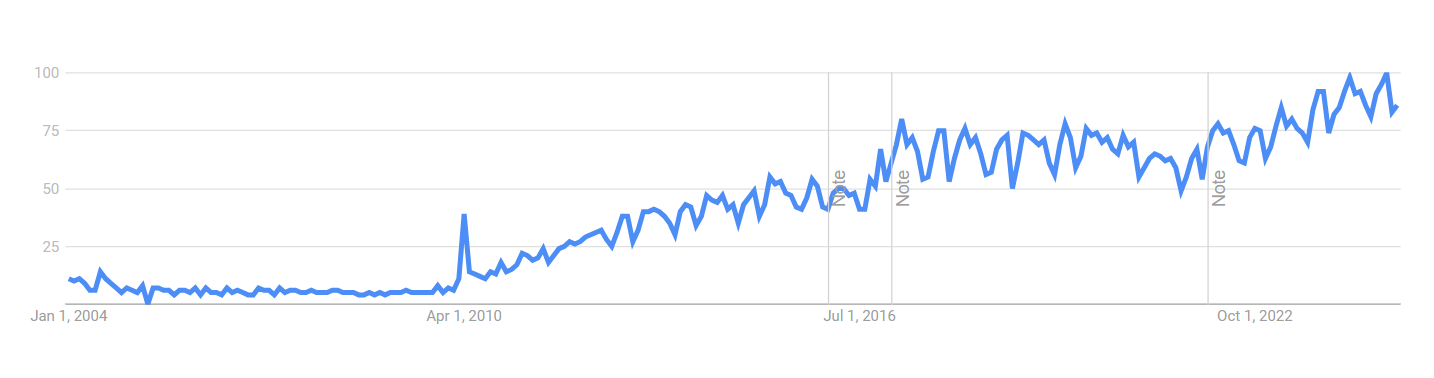
\includegraphics[width=\textwidth]{open_data_google_trends}
    \caption[Open Data su Google Trends]{Ricerche su Google relative al termine Open Data effettuate dal 2004 al 2025. Notare l'aumento successivo al 2009 e il trend in crescita \cite{Google_Trends}.}
    \label{fig:open_data_google_trends}
\end{figure}

\subsection{Concetto di Open Data}
%Definizione e principi fondamentali
Gli \textit{open data}, specialmente quelli della pubblica amministrazione, costituiscono una formidabile risorsa che ancora oggi rimane in larga parte inutilizzata. Molte persone e organizzazioni raccolgono una vasta gamma di svariati tipi di dati per svolgere le proprie attività. In questo ambito, il governo riveste particolare importanza, sia per la quantità e la centralità dei dati che raccoglie, sia perché la maggior parte dei dati del governo sono pubblici per legge, quindi potrebbero diventare aperti e resi disponibili per l'utilizzo da parte di chiunque. Questo riveste particolare interesse in quanto si ritiene che gli \textit{open data} possano apportare benefici in molti settori, ed esistono altrettanti esempi di come siano già stati usati con successo. Ci sono inoltre svariati gruppi di persone e organizzazioni che possono trarre vantaggi dalla disponibilità di \textit{open data}, incluso il governo stesso. Allo stesso tempo, è impossibile effettuare previsioni esatte su come e dove verranno apportati questi benefici in futuro, in quanto è nella stessa natura dell'innovazione che gli sviluppi spesso partano dai posti più inaspettati \cite{OpenDataHandbook_WhyOpenData}.

\subsection{Caratteristiche principali degli Open Data}
% Accessibilità, Interoperabilità, Riutilizzabilità
% Formati comuni: CSV, JSON, XML
In base a quanto stabilito dalla \textit{Open Definition}, gli \textit{open data} sono dati che possono essere utilizzati liberamente e ridistribuiti da chiunque e sono sottoposti, al massimo, al riconoscimento obbligatorio di una potenziale attribuzione o crediti in generale \cite{OpenDefinition}. Nella \textit{full Open Definition} vengono specificate in dettaglio le proprietà più importanti, ovvero:

\begin{itemize}
    \item \textbf{Disponibilità e Accesso:} i dati devono essere disponibili per intero, senza pagare più di un costo ragionevole di riproduzione, preferibilmente scaricandoli dalla rete Internet. I dati devono, inoltre, essere disponibili in un formato conveniente e modificabile.
    \item \textbf{Riutilizzo e Ridistribuzione:} i dati devono essere forniti sotto licenza che ne permetta liberamente il riutilizzo e la ridistribuzione, incluso specialmente il mescolamento con altri \textit{dataset}.
    \item \textbf{Partecipazione Universale:} tutti devono essere in grado di utilizzare, riutilizzare e ridistribuire i dati, senza discriminazioni contro campi di applicazione o contro persone o gruppi particolari. Ad esempio, non sono permesse le licenze ristrette ai soli scopi non-commerciali, che impedirebbero l'utilizzo commerciale, e nemmeno qualsiasi altra restrizione all'uso per certe finalità, come quella esclusivamente educativa.
\end{itemize}

Queste regole sono necessarie per garantire chiarezza sul significato di apertura e, soprattutto, per assicurarne l'\textit{interoperabilità}. Quest'ultima denota la capacità di lavorare insieme, ovvero interoperare, tra diversi sistemi e organizzazioni, che in questo caso si riferisce all'interoperabilità, detta anche mescolanza, tra dataset differenti. \`E una capacità molto importante perché permette a diversi componenti di collegarsi per lavorare insieme e questo è essenziale per realizzare sistemi grandi e complessi, la cui costruzione altrimenti sarebbe quasi impossibile senza interoperabilità \cite{OpenDefinition_Full}.

Il principio cardine di un \textit{commons} di dati o codice, ovvero una raccolta di essi, è che un qualunque pezzo di materiale aperto lì contenuto possa essere mescolato liberamente con altro materiale aperto. Questa interoperabilità è assolutamente necessaria a livello pratico per realizzare i principali benefici ottenibili dall'apertura dei dati, ovvero l'abilità notevolmente migliorata di combinare insieme diversi dataset e di conseguenza la capacità di sviluppare un numero maggiore di prodotti e servizi aventi qualità migliore. Questa definizione data riguardo all'apertura assicura che, dati due dataset aperti ottenuti da due fonti diverse, possiamo essere sempre in grado di combinarli insieme, evitando di trovarci di fronte a un numero enorme di dataset aventi scarsa o nulla capacità di essere mescolati insieme in sistemi di più larga scala, senza quindi avere la capacità di apportare valore aggiunto. Il punto chiave di aprire i dati deve essere il \textit{focus} su dati non-personali, ovvero i dati non devono contenere informazioni riguardanti persone specifiche. Inoltre, per alcuni tipi di dati ottenuti dal governo, potrebbero applicarsi restrizioni nazionali per motivi di sicurezza \cite{OpenDataHandbook_WhyOpenData}.

\subsection{Confronto con dati privati}
Differenze principali

Vantaggi e svantaggi rispetto agli Open Data

\subsection{Contesto italiano e internazionale}
Ad oggi, è già possibile indicare un cospicuo numero di settori nei quali i dati aperti del governo stanno già apportando un certo valore, tra cui:

\begin{itemize}
    \item Controllo di trasparenza e democrazia.
    \item Partecipazione.
    \item Autopotenziamento.
    \item Miglioramento o creazione di nuovi prodotti e servizi da parte di privati.
    \item Innovazione.
    \item Miglioramento dell'efficienza di servizi del governo.
    \item Miglioramento dell'efficacia di servizi governativi.
    \item Misuramento dell'impatto di certe politiche.
    \item Nuova conoscenza ottenuta dalla combinazione di fonti di dati e dalla ricerca di \textit{pattern} all'interno di grandi volumi di dati.
\end{itemize}

Riguardo alla trasparenza, esistono progetti come il finlandese \textit{tax tree}, l'albero delle tasse, e il britannico \textit{where does my money go}, dove vanno i miei soldi, per visualizzare in che modo i ricavi derivanti dalle tasse vengono spesi dal governo. Inoltre, possiamo ricordare come gli open data abbiano risparmiato al Canada \$3.2 miliardi in una frode fiscale relativa a un ente di beneficenza. Altri siti web includono il danese \textit{folketsting.dk} per tracciare l'attività in parlamento e i processi di creazione di leggi, così da poter vedere esattamente gli eventi che stanno accadendo, e quali parlamentari sono coinvolti.
Gli open data del governo possono anche aiutarci a prendere decisioni migliori nella nostra vita, o a diventare più attivi nella società. Una donna in Danimarca ha sviluppato \textit{findtoilet.dk}, che mostra tutti i bagni pubblici danesi così che le persone che conosceva con problemi alla vescica potessero diventare più sicuri di se stessi quando andavano nuovamente fuori. In Olanda è disponibile un servizio, \textit{vervuilingsalarm.nl}, che ci avvisa con un messaggio se domani la qualità dell'aria nelle vicinanze raggiungerà una soglia che abbiamo definito in precedenza. A New York possiamo facilmente capire dove possiamo portare il cane a passeggio, insieme a trovare altre persone che frequentano gli stessi parchi. Servizi come \textit{mapumental} nel Regno Unito e \textit{mapnificent} in Germania permettono di trovare dei posti in cui vivere, prendendo in considerazione la durata del tragitto per arrivare a lavoro, il prezzo delle case e la qualità di una certa zona. Tutti questi servizi, per funzionare, si appoggiano a dati forniti apertamente dal governo.
Economicamente, gli open data sono altrettanto importanti: diversi studi hanno stimato il valore economico degli open data in alcune decine di miliardi di Euro su base annua, e questo solamente nell'Unione Europea. Nuovi prodotti e aziende stanno riutilizzando dati aperti, come ad esempio il danese \textit{husetsweb.dk} che aiuta a trovare dei modi per migliorare l'efficienza energetica della propria casa, insieme alla pianificazione finanziaria e alla ricerca di costruttori che possano svolgere il lavoro. Tutto è basato sul riutilizzo delle informazioni catastali e informazioni sui sussidi da parte del governo, insieme al registro commerciale locale. Google Traduttore utilizza un enorme quantità di documenti dell'UE che compaiono in tutte le lingue europee per addestrare gli algoritmi di traduzione e quindi migliorare la sua qualità del servizio.
Gli open data offrono del valore anche al governo stesso, ad esempio per aumentarne l'efficienza. Il Ministero Olandese dell'Istruzione ha pubblicato online tutti i suoi dati relativi all'istruzione, permettendone il riuso. Da allora, il numero di domande che hanno ricevuto è crollato, riducendo il carico di lavoro e i relativi costi, mentre per i dipendenti pubblici è più facile rispondere alle rimanenti domande, in quanto diventa maggiormente chiaro dove possono essre trovate le informazioni rilevanti. Gli open data hanno anche reso più efficiente la pubblica amministrazione, il che porta a un'ulteriore riduzione dei costi. Il dipartimento olandese dei beni culturali sta rilasciando attivamente i loro dati e collabora con società amatoriali di storia e gruppi come la \textit{Wikimedia Foundation} per eseguire i loro compiti in maniera più efficiente. Questo non solo porta a miglioramenti nella qualità dei loro dati, ma contribuisce anche a rimpicciolire le dimensioni del dipartimento stesso.
Anche se ci sono già numerose istanze relative ai modi in cui gli open data stanno creando del valore aggiunto sia in ambito sociale che in quello economico, non sappiamo ancora nulla riguardo alle nuove cose che diventeranno possibili. Nuove combinazioni di dati possono creare ulteriore conoscenza, il che può potenzialmente portare a scoprire campi di applicazione completamente nuovi. Lo abbiamo già visto in passato, per esempio quando nel XIX secolo a Londra il Dott. Snow ha scoperto il legame tra inquinamento dell'acqua potabile e colera, combinando i dati delle morti attribuibili al colera con la posizione dei pozzi d'acqua. Questo portò alla costruzione dei sistemi fognari di Londra e migliorò notevolmente la salute pubblica della popolazione. Probabilmente potremmo vedere accadere nuovamente degli sviluppi simili, scaturiti dalla combinazione di diversi dataset aperti. Questo potenziale, ancora non sfruttato, può essere rilasciato se trasformiamo i dati pubblici del governo in open data, ma solo se sono davvero aperti, ovvero se non sottoposti ad alcun tipo di restrizione legale, finanziaria o tecnologica relativa al suo riutilizzo da parte di terzi. Ogni restrizione impedisce alle persone di riutilizzare i dati pubblici, o quantomeno lo rende più difficile. Per poter realizzare appieno il loro potenziale, i dati pubblici devono essere aperti, ovvero degli open data \cite{OpenDataHandbook_WhyOpenData}.

\subsubsection{Iniziative globali}
Open Government Partnership

\subsubsection{Normativa italiana}
CAD (Codice dell'Amministrazione Digitale)

\subsubsection{Portali di Open Data}
dati.gov.it

Open Data Bologna (https://opendata.comune.bologna.it/)

\subsubsection{Casi studio e iniziative significative}
INSPIRE

Copernicus


\section{Bologna e progetto BolognaWiFi}  %  e Comune di Bologna
\subsection{Bologna Smart City}
\subsubsection{Digitalizzazione e innovazione urbana}
Progetti principali

\subsubsection{Politiche locali per gli Open Data}
Strategie e risultati

\subsubsection{Infrastrutture digitali recenti}
Implementazioni chiave

\subsection{Progetto BolognaWiFi}
\subsubsection{Obiettivi principali}
Scopi e finalità del progetto

\subsubsection{Tipologie di dati raccolti}
Flussi utenti

Accessi WiFi

Affluenza in aree urbane

\subsubsection{Statistiche recenti}
Dati sull'uso del WiFi pubblico a Bologna

\subsubsection{Risorse utili}
Documentazione ufficiale del progetto

Report e analisi pubblicati dal Comune


\section{Visualizzazione dei dati}  % Analisi e
\subsection{Importanza della visualizzazione}
\subsubsection{Analisi dei dati urbani}
Esempi pratici e benefici

\subsubsection{Supporto decisionale}
Impatti sulle amministrazioni pubbliche

\subsection{Caratteristiche di una buona visualizzazione}
Chiarezza e semplicità

Interattività e Accessibilità

\subsection{Strumenti di visualizzazione}
\subsubsection{Panoramica degli strumenti comuni}
Tableau

D3.js

\subsubsection{Vantaggi e svantaggi degli strumenti}
Breve descrizione comparativa

\subsubsection{Applicazioni pratiche}
Esempi nelle smart cities


\section{Sfide e opportunità}   % Benefici e potenziale degli Open Data
\subsection{Sfide tecniche}
\subsubsection{Gestione di dataset eterogenei}
Problemi e soluzioni

\subsubsection{Scalabilità e performance}
Tecnologie per ottimizzare

\subsection{Aspetti etici e legali}
\subsubsection{Privacy e anonimizzazione dei dati}
Strumenti e tecniche utilizzate

\subsubsection{Licenze e diritti d'uso}
Regolamenti e pratiche comuni

\subsubsection{Casi noti di violazioni}
Esempi significativi e lezioni apprese

\subsection{Opportunità}
\subsubsection{Trasparenza e coinvolgimento}
Benefici per cittadini e istituzioni

\subsubsection{Pianificazione urbana}
Utilizzo dei dati per migliorare i servizi

\subsubsection{Collaborazioni pubblico-privato}
Partnership per sfruttare al meglio gli Open Data

\subsection{Fonti per approfondire}
\subsubsection{Linee guida GDPR}
Applicazioni rilevanti per i dati urbani

\subsubsection{Studi accademici}
Temi su etica e Open Data